% !TEX root = ./Vorlesungsmitschrift DIFF 2.tex  
\lecture{Do 23.04. 10:15}{} Bevor wir uns mit offenen und abgeschlossenen Mengen und
sogenannten vollständigen metrischen Räumen näher befassen, beweisen wir noch zwei
nützliche Lemmata zu Konvergenz und Stetigkeit:

\begin{lemma}\label{konvergenz_abstand_ist_nullfolge}
    \( (X,d) \) sei metrischer Raum.

    Eine Folge \( (x_n)_n \) in \( X \) konvergiert in \( X \) gegen \( a\in X \)
    \begin{align*}
        \iff (\distance{x_n}{a})_n \text{ ist Nullfolge}\logicspace(\text{in } \reals).
    \end{align*}
\end{lemma}
\begin{proof}
    \begin{align*}
        \distance{x_n}{a}=\abs{\distance{x_n}{a}-0}.
    \end{align*}
    Also ist
    \begin{align*}
        \distance{x_n}{a}<\varepsilon\iff \abs{\distance{x_n}{a}-0}<\varepsilon.
    \end{align*}
    
\end{proof}
\begin{lemma}\label{stetigkeit:folgenkonvergenzkriterium}
    Seien \( (X,d_x) \) und \( (Y, d_y) \) metrische Räume, \( f\maps X\to Y \) eine Abbildung. 
    Dann gilt:

    \( f \) ist in \( a\in X \) stetig \tiff für jede Folge \( (a_n)_n \) mit \( a_n\goesto a \) in \( X \) gilt
    \begin{align*}
        \lim\limits_{n \goesto \infty}  f(a_n)=f(\underbrace{\lim a_n}_{=a}).
    \end{align*} 
    \begin{notation*}
        \begin{align*}
            \lim\limits_{x \goesto a} f(x)=f(a).
        \end{align*}
    \end{notation*}
    
\end{lemma}
\begin{proof}
    \begin{proofdescription}
        
        \item[\hin] Sei das \( \varepsilon \)-\( \delta \)-Kriterium erfüllt (\ref{stetigkeit_in_metrischen_raeumen}).
        Sei \( (x_n)_n \) Folge in \( X \) mit \( x_n\goesto a \) in \( X \). Sei \( \varepsilon>0 \). Dann \texists \( \delta>0 \) \sd
        \begin{align*}
            d_Y(f(x),f(a))<\varepsilon\logicspace\forall x\in \ball{\delta}{a}\subset X.
        \end{align*} 
        Wegen der Konvergenz \texists \( N=N(\delta) \) \sd
        \begin{align*}
            &x_n\in \ball{\delta}{a} \logicspace\forall n\geq N\\
            \implies &f(x_n)\in B_\varepsilon(f(a))\subset Y \logicspace \forall n\geq N.
        \end{align*}
        Also gilt \( f(x_n)\goesto f(a) \).
        \item[\rueck] Gelte \( \lim_{x \goesto a} (x)=f(a) \).
        
        Angenommen, das \( \varepsilon \)-\( \delta \)-Kriterium wäre verletzt. Dann gäbe es \( \varepsilon>0 \) \sd für \emph{alle} \( \delta>0 \) ein \( x\in X \) existierte \sd
        \begin{align*}
            x\in \ball{\delta}{a}\logicspace \begin{aligned}[t] 
                &\text{aber} \logicspace f(x)\notin B_\varepsilon(f(a))\\
                &\text{also} \logicspace d_y(f(x), f(a)) \geq \varepsilon.
            \end{aligned}
        \end{align*}
        Insbesondere gäbe es zu \( \delta=\frac{1}{n} \) ein solches \( x \), nennen wir es \( x_n \). Dann gilt für alle \( n \): \( \distance{x_n}{a}<\frac{1}{n} \), aber \( d_y(f(x_n),f(a))\geq \varepsilon \), somit \( x_n\goesto a \) aber \( f(x_n)\not\goesto f(a) \) (wegen \ref{konvergenz_abstand_ist_nullfolge}).
    \end{proofdescription}
    
    
\end{proof}
\section{Charakterisierung topologischer Grundbegriffe in metrischen Räumen}
\begin{lemma}\label{abgeschlossenheit:folgenkonvergenzkriterium}
    Sei \( (X,d) \) metrischer Raum. 
    Dann ist \( A\subset X \) abgeschlossen \tiff für jede Folge \( (a_n)_n \), \( a_n\in A \), die in \( X \) konvergiert, gilt:
    \begin{align*}
        \lim\limits_{n \goesto \infty} a_n\in A.
    \end{align*}
\end{lemma}
\begin{proof}
    \Obda \( \emptyset\neq A\neq X \).
    
    \begin{proofenumerate}
        
        \item[\hin] Sei \( (a_n)_n \), \( a_n\in A \), konvergent in \( X \).
         Sei \( a=\lim a_n \). Angenommen \( a\notin A \). Nach Voraussetzung ist \( X\setminus A \) offen, also ist \( X\setminus A \) Umgebung von \( a \) \timplies \texists \( N \) \sd
         \begin{align*}
             a_n \in X\setminus A \logicspace \forall n\geq N \logicspace (\text{wegen Konvergenz})
         \end{align*}
         \contra zu \( a_n\in A \).
         
         \item[\rueck] Wir zeigen, dass \( X\setminus A \) offen ist.
         Sei also \( b\in X \setminus A \). Es gibt \( \varepsilon>0 \) \sd \( \ball{\varepsilon}{b}\cap A=\emptyset \), also \( \ball{\varepsilon}{b}\subset X\setminus A \). 
         
         Denn angenommen es gibt kein solches \( \varepsilon \). 
         Dann gilt für \emph{alle} \( \varepsilon>0 \):
         \( \ball{\varepsilon}{b}\cap A\neq \emptyset \), also kann man zu jedem \( k\geq 1 \) ein \( x_k\in A \) finden mit \( \distance{x_k}{ b}<\frac{1}{k}=\varepsilon \).
         \begin{align*}
             \implies x_k=b\underset{\text{\textsc{Vor}}}{\implies} b\in A.
         \end{align*}
         \contra Wiederspruch zu \( b\in X\setminus A \).

         Also gibt es ein solches \( \varepsilon>0 \), also ist \( X\setminus A \) offen.
    \end{proofenumerate}
    
\end{proof}
\begin{definition}\index{Randpunkt}
    Sei \( (X,d) \) metrischer Raum, \( M\subset X \). Ein Punkt \( y\in X \) heißt \emph{Randpunkt} von \( M \), falls in jeder Umgebung von \( y \) sowohl Punkte von \( M \) als auch \( X\setminus M \) liegen.
\end{definition}
\begin{notation*}
    \( \randpunkte{M}=\Set{\text{Randpunkte von \( M \)}} \)
\end{notation*}
\begin{beispiel*}[\( \reals^n \), \( d_{\text{Eukl.}} \)]
   Kugel im \( \reals^m \):
   \begin{align*}
       K^n&\definedas \Set{x\in \reals^n| \norm{x-0}_\text{E}\leq R}\subset \reals^n\\
       \intertext{Sphäre:}
       \randpunkte{K^n} &=\Set{x\in \reals^n|\norm{x}_\text{E}= R}=S^{n-1}
   \end{align*} 
\end{beispiel*}

\begin{beispiel*}
    \( \rationals\subset \reals \). \( \randpunkte{\rationals} =\reals\).
\end{beispiel*}
\begin{satz}
    Sei \( (X,d) \) metrischer Raum. Sei \( M\subset X \). Dann gilt
    \begin{enumerate}
        \item \label{interior_ist_offen}\( M\setminus \randpunkte{M} \) ist offen.
        \item \label{abschluss_ist_geschlossen}\( M\cup \randpunkte{M} \) ist abgeschlossen.
        \item \label{rand_ist_geschlossen}\( \randpunkte{M} \) ist abgeschlossen.
    \end{enumerate}
\end{satz}
\begin{proof}
    \begin{proofdescription}
        \item[\ref{interior_ist_offen}:] \( a\in M\setminus \randpunkte{M} \) \timplies \texists \( \varepsilon>0 \) \sd \( \ball{\varepsilon}{a}\cap X\setminus M = \emptyset \). Für dieses gilt auch \( \ball;{\varepsilon}\cap \randpunkte{M}=\emptyset\) (denn angenommen \texists \( y\in \ball{\varepsilon}{a} \cap \randpunkte{M} \),  dann wäre (da \( y\in \randpunkte{M} \) und \( \ball{\varepsilon}{a} \) eine Umgebung von \( y \)) \( \ball{\varepsilon}{a}\cap (X\setminus M)\neq \emptyset \) \contra \textsc{VOR}).
        
        Also gilt \( \ball{\varepsilon}{a}\subset M\setminus \randpunkte{M} \) \timplies \Beh.
        \item[\ref{abschluss_ist_geschlossen}:] Es gilt \( \randpunkte{M}=\randpunkte{X\setminus M} \) (nach Definition), \( (X\setminus M)\setminus \randpunkte{X\setminus M} \) ist offen nach \ref{interior_ist_offen} \timplies \begin{align*}
            X\setminus ((X\setminus M)\setminus \randpunkte{X\setminus M})\explain{\text{Manipulation mit Mengen}}{=}(X\setminus(X\setminus M))\cup \randpunkte{X\setminus M}=M\cup \randpunkte{M}
        \end{align*}
        ist offen.
        \begin{figure}[H]
            \centering
            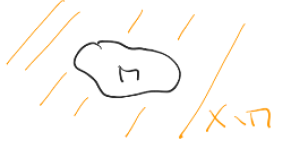
\includegraphics[width=0.5\linewidth]{figures/menge_und_komplement}
            \label{fig:menge_und_komplement}
        \end{figure}
        \item[\ref{rand_ist_geschlossen}:]
        \begin{align*}
            &\randpunkte{M}=(M\cup \randpunkte{M})\setminus (M\setminus \randpunkte{M})\\
            \implies &X\setminus \randpunkte{M}=\underbrace{X\setminus(\underbrace{M\cup \randpunkte{M}}_{\text{(abgeschl.\ nach \ref{abschluss_ist_geschlossen})}})}_{\text{offen}}\cup (\underbrace{M\setminus \randpunkte{M}}_{\text{offen nach \ref{interior_ist_offen}}}).
        \end{align*} 
    \end{proofdescription}
\end{proof}

\begin{notation*}
    Sei \( M\subset X \).
    \begin{align*}
        \inneres{M}&\definedas M\setminus \randpunkte{M}\text{ heißt das \emph{Innere} von \( M \).}\\
        \abschluss{M}&\definedas M\cup \randpunkte{M}\text{ heißt der \emph{Abschluss} von \( M \).}
    \end{align*}
\end{notation*}
Nach \ref{abgeschlossenheit:folgenkonvergenzkriterium} können wir \( \abschluss{M} \) konstruieren, indem wir zu \( M \) noch alle Grenzwerte von Folgen \( (x_n)_n \), \( x_n\in M \), die in in \( X \) konvergieren, hinzunehmen.
\begin{beispiel*}
    \( M=\rinterval{a}{b} \), \( \abschluss{M}=\interval{a}{b} \).
\end{beispiel*}
\begin{bemerkung*}[als Hausaufgabe]
    \begin{align*}
        M&\subset X \text{ offen} \iff M\cap \randpunkte{M}=\emptyset.\\
        M&\subset X \text{ abgeschlossen} \iff \randpunkte{M} \subset M.
    \end{align*}
    
\end{bemerkung*}
\section{Vollständigkeit}
\begin{definition}\index{Cauchy-Folge}
    Sei \( (X,d) \) ein metrischer Raum. Eine Folge \( (y_n)_n \subset X\) heißt \emph{Cauchy-Folge}, falls gilt
    \begin{align*}
        \forall \varepsilon>0 \logicspace \exists N\in \naturals \logicspace\text{\sd}\logicspace \distance{y_n}{ y_m}<\varepsilon \logicspace \forall n,m\geq N.
    \end{align*} 
\end{definition}
\begin{lemma}
    Sei \( (X,d) \)  ein metrischer Raum. Eine konvergente Folge in \( X \)  ist eine \emph{Cauchy-Folge}.
\end{lemma}
\begin{proof}
    Sei \( (y_n)_n \)  konvergente Folge mit Grenzwert \( y \) (eindeutig wegen \ref{metrischer_raum_ist_hausdorffsch} und \ref{hausdorff_alle_grenzwerte_eindeutig}). Sei \( \varepsilon>0 \).

    Dann gibt es \( N\in \naturals  \) \sd \( \distance{y_m}{ y}<\varepsilon \logicspace  \forall m\geq N\).
    \begin{align*}
        \implies \distance{y_n}{y_m}\underset{\triangle}{\leq}\distance{y_n}{y}+\distance{y}{y_m}<\epsilon \logicspace \forall n,m\leq N.
    \end{align*}   
\end{proof}
\begin{bemerkung*}
    Nicht jede Cauchy-Folge konvergiert:
    \begin{beispiel*}[\((\rationals, \abs{\cdot} )\)]
        \( y_{n+1}=\frac{1}{2}y_n+\frac{1}{y_n} \), \( y_0=1 \). 
    \end{beispiel*}
    \begin{checkenvironment*}
        Es gilt für \( n\geq 1 \)
        \begin{align*}
            \interval{\frac{1}{y_{n+1}}}{y_{n+1}}\subset \interval{\frac{1}{y_n}}{y_n} \label{eq:cauchy_folge_konvergiert_nicht:beispiel:intervallschachtelung}\tag{\(*\)}
        \end{align*} 
        und für \( l_n\definedas y_n-\frac{1}{y_n} \) 
        \begin{align*}
            &l_{n+1}\leq\frac{1}{4y_{n+1}}l_n^2\leq \frac{1}{4}l_n^2\tag{\(**\)}\label{eq:cauchy_folge_konvergiert_nicht:beispiel:abstand_nullfolge}\\
            \implies &\distance{y_n}{y_m}=\abs{y_n-y_m} \explain{\substack{\text{\Obda\ }m\geq n\\\implies y_m\in \interval{\frac{1}{y_n}}{y_n} \text{ wg.\ \eqref{eq:cauchy_folge_konvergiert_nicht:beispiel:intervallschachtelung}}}}{\leq}\abs{y_n-\frac{1}{y_n}}=l_n\explain{\text{wg.\ \eqref{eq:cauchy_folge_konvergiert_nicht:beispiel:abstand_nullfolge}}}{\goesto} 0.
        \end{align*}
        \( \rationals \subset \reals  \)  und somit \( (y_n)_n \subset \reals \).
        In \( \reals \) konvergiert jede Cauchy-Folge.
        Nennen wir den Grenzwert \( a\in \reals \). Es gilt dann
        \begin{align*}
            \underbrace{y_{n+1}}_{\goesto a}=\underbrace{\frac{1}{2}y_n}_{\frac{1}{2}a}+\underbrace{\frac{1}{y_n}}_{\frac{1}{a}},
        \end{align*} 
        also \( a^2=2\). Aber \( \sqrt{2}\notin \rationals \).
    \end{checkenvironment*}
    
\end{bemerkung*}
\begin{definition}\index{Vollständiger metrischer Raum}
    Ein metrischer Raum, in dem jede Cauchy-Folge konvergiert heißt \emph{vollständig}.
\end{definition}
\begin{beispiele}
    \begin{enumerate}
        
        \item \label{r_ist_vollstaendig} \( \reals ,\abs{\cdot} \) ist vollständig (\diffcourse{1}).
        \item \label{integral_metrischer_raum_ist_nicht_vollstaendig} \( (\stetigefunktionen(\interval{a}{b} ,\reals), d_{L^1})\) mit \( d_{L^1}(f,g)=\Integrate{\abs{f(t)-g(t)}}{t,a,b}\) (\vgl HA Blatt 1, A1) ist \emph{nicht} vollständig. 
        \item \( (\stetigefunktionen(\interval{a}{b},\reals ), d_{\sup})\), mit
        \begin{align*}
            d_{\sup}=\supnorm{f-g}=\sup_{t\in \interval{a}{b}}\abs{f(t)-g(t)},
        \end{align*}
        ist vollständig.
        Den Beweis führen wir später allgemeiner.
    \end{enumerate}
    

\end{beispiele}
Zunächst einige 
\section{Betrachtungen in vollständigen metrischen Räumen}

\begin{definition}\index{Beschränktheit}
    Sei \( (X,d)\) metrischer Raum, \( M\subset X\),
    \begin{align*}
        \diameter{M}\definedas \sup_{x,y\in M}\distance{x}{y}\logicspace \text{\enquote{Durchmesser} (englisch \enquote{diameter})}.
    \end{align*}
    \( M \) heißt \emph{beschränkt}, falls \( \diameter{M}<\infty \).
\end{definition}
\begin{bemerkung*}
    \( M\) ist beschränkt \tiff \texists \( R\geq 0\)  und \( a\in X\) \sd \( M\subset \ball{R}{a}\) 
    \begin{figure}[H]
        \centering
        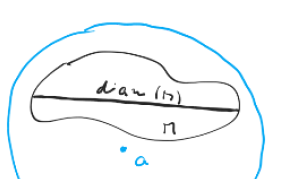
\includegraphics[width=0.5\linewidth]{figures/beschraenkte_menge_in_ball}
        \label{fig:beschraenkte_menge_in_ball}
    \end{figure}   
\end{bemerkung*}
\begin{beispiel*}
    \( \diameter{\rinterval{a}{b}}=b-a\)
\end{beispiel*}
\begin{satz}[Schachtelungsprinzip]\index{Schachtelungsprinzip}
    Sei \( (X,d)\) ein \emph{vollständiger} metrischer Raum und sei \( A_0\subset A_1\subset A_2\subset \cdots\).
    Eine Familie nicht-leerer abgeschlossener Teilmengen von \( X\) mit
    \begin{align*}
        \diameter{A_k}\goesto 0 \logicspace (\text{in }\reals)\logicspace \text{für } k\goesto \infty. 
    \end{align*} 
    Dann gibt es genau einen Punkt \( a\in X\) der in \emph{allen} \( A_k\) liegt.
\end{satz}
\begin{proof}
    \begin{proofdescription}
        \item[Eindeutigkeit:] Angenommen \texists \( x\neq y\)  mit \( x\in A_k \logicspace \forall k\)  und \( y\in A_k \logicspace \forall k\). Dann kann \( \diameter{A_k}\) keine Nullfolge sein, da \( \distance{x}{y}\neq 0\).
        \item[Existenz:] Wähle \( x_n\in A_n\). Dann ist \( (x_n)_n\)  eine Cauchy-Folge, denn
        \begin{align*}
            \distance{x_n}{x_m}\leq \diameter-{A_N} \logicspace \text{für }n,m\geq N 
        \end{align*} 
        \begin{figure}[H]
            \centering
            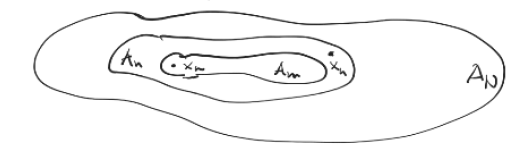
\includegraphics[width=0.5\linewidth]{figures/schachtelungsprinzip}
            \caption*{\( \distance{x_n}{x_m}\leq \diameter-{A_N}\) für \( \)    }
            \label{fig:schachtelungsprinzip}
        \end{figure}
        \begin{align*}
            \explain{\text{Vollständigkeit}}{\implies}x_n \goesto x \logicspace \text{in } X,
        \end{align*}
        Da \( x_n\in A_k\logicspace \forall n\geq k\), folgt mit \ref{abgeschlossenheit:folgenkonvergenzkriterium}: \( x\in A_k\logicspace \forall k\). 
    \end{proofdescription}
\end{proof}
Ein sehr wichtiger Satz, der viele Anwendungen hat ist der folgende:
\begin{satz}[Banach'scher Fixpunktsatz]\index{Banach'scher Fixpunktsatz}
    Sei \( (X,d_X)\) ein \emph{vollständiger} metrischer Raum. Sei \( M\subset X\) eine \emph{abgeschlossene} Teilmenge und \( \Phi\maps M\to X\) eine Abbildung mit \( \Phi(M)\subset M\) und es gebe \( 0\leq L<1\) \sd
    \begin{align*}
        d_X(\Phi(x),\Phi(y))\leq L d_X(x,y)\logicspace\forall x,y\in M\logicspace (\text{\enquote{\( \Phi\) ist Kontraktion}}).
    \end{align*}
    Dann gibt es genau ein \( t_*\) \sd \( \Phi(t_*)=t_*\). Ein solches \( t_*\) heißt \emph{Fixpunkt} von \( \Phi\). 
\end{satz}
\begin{beispiel*}
    \begin{figure}[H]
        \centering
        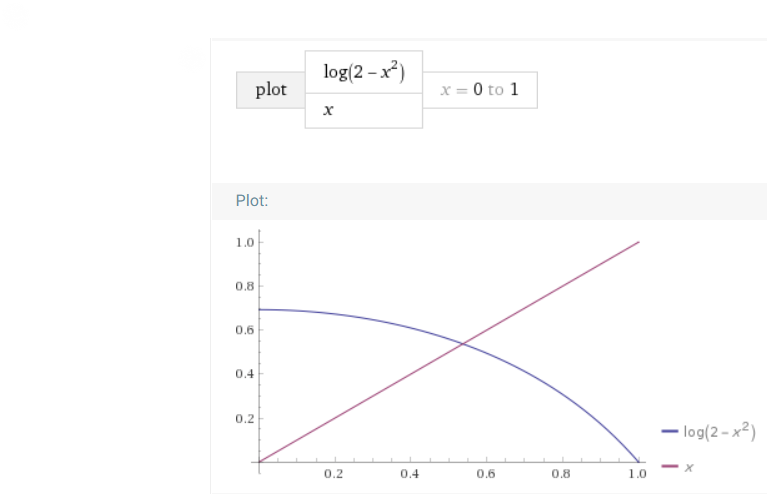
\includegraphics[width=0.5\linewidth]{figures/fixpunkt_beispiel}
        \caption*{\( X=\reals \), \( M=\interval{0}{1} \), \( \log(2-x^2)\), (WolframAlpha)}
        \label{fig:fixpunkt_beispiel}
    \end{figure}
\end{beispiel*}
\begin{proof}
    \begin{proofdescription}
        \item[Eindeutigkeit:] Seien \( \Phi(t_*)=t_*\), \( \Phi(\tilde{t}_*)=\tilde{t}_* \). Dann gilt
        \begin{align*}
            \distance{t_*}{\tilde{t_*} }\begin{aligned}[t]
                &=\distance{\Phi(t_*)}{\Phi(\tilde{t}_*)}\\
                &\leq \distance{t_*}{\tilde{t_*} }
            \end{aligned}
        \end{align*} 
        Da \( L<1\) ist, folgt \( \distance{t_*}{\tilde{t_*}=0 }\), also \( t_*=\tilde{t_*} \).
        \item[Existenz:] Wir betrachten die Folge \( x_0\in M\) beliebig, \( x_n\definedas \Phi(x_{n-1})\) für \( n\geq 1\).
        \begin{behauptung*}
            \( (x_n)_n\) konvergiert in \( M\)  und zwar gegen de Fixpunkt.
        \end{behauptung*}
        \begin{subproof}
            \begin{itemize}
                \item \( (x_n)_n\) ist Cauchy-Folge:
                \begin{align*}
                    \distance{\equalto{\Phi(x_n)}{x_{n+1}}}{\equalto[Bigg]{\Phi(x_{n-1})}{x_n}}\leq L \distance{x_n}{x_{n-1}}\logicspace \forall n\geq 1.
                \end{align*}
                Iteration liefert
                \begin{align*}
                    \distance{x_{n+1}}{x_n}\leq L^2 \distance{x_{n-1}}{x_{n-2}}\leq \cdots \leq L^n \distance{x_1}{x_0}.
                \end{align*}
                Zudem gilt
                \begin{align*}
                    \distance{x_{n+k}}{x_n}\begin{aligned}[t]
                        &\underset{\triangle}{\leq}\begin{aligned}[t]
                            &\distance{x_{n+k}}{x_{n+k}-1}\\
                            &+\distance{x_{n+k-1}}{x_{n+k-2}}\\
                            &\vdots\\
                            &+\distance{x_{n+1}}{x_n}
                        \end{aligned}\\
                        &\leq (\underbrace{L^{n+k-1}+L^{n+k-2}+\cdots+L^n}_{\mathclap{=L^n \sum_{r=0}^{k-1} L^r\leq L^n \sum_{r=0}^{\infty} L^r\explain{\text{geom.\ Reihe (\( L<1\))}}{=}\frac{L^n}{1-L}}})\distance{x_1}{x_0}
                    \end{aligned}
                \end{align*}
                \timplies (wegen \( L<1\)) \Beh.
                
                \item Da \( X\) vollständig ist, konvergiert \( (x_n)_n\). Setze \( t_*=\lim\limits_{n \goesto \infty} x_n\).
                \item Da \( M\) abgeschlossen ist, ist \( t_*\in M\) nach \ref{abgeschlossenheit:folgenkonvergenzkriterium}.
                \item \( t_*\) ist der gesuchte Fixpunkt:
                \begin{align*}
                    t_*=\lim\limits_{n \goesto \infty} x_n=\lim\limits_{n \goesto \infty} \Phi(x_{n-1})\explain{\text{Kontraktionen sind stetig und \ref{stetigkeit:folgenkonvergenzkriterium}}}{=}\Phi(t_*)
                \end{align*} 
            \end{itemize}
        \begin{figure}[H]
            \centering
            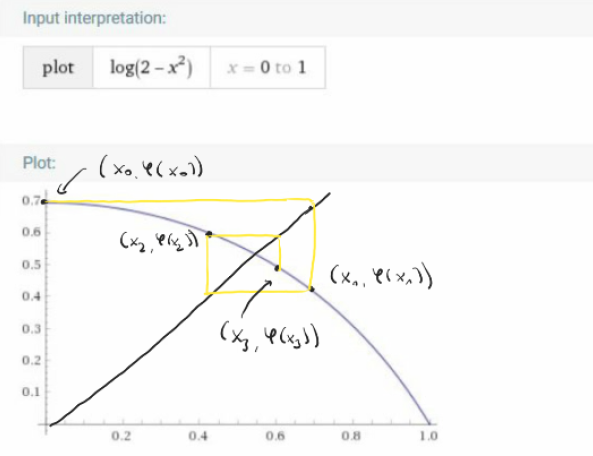
\includegraphics[width=0.6\linewidth]{figures/fixpunktsatz_beweis_existenz}
            \caption*{\( x_0=0\), \( x_1\Ln+{2-(\Ln{2})^2}\approx 0,42\), \( x_3\approx 0,60\), \( x_4\approx 0,49\)}
            \label{fig:fixpunktsatz_beweis_existenz}
        \end{figure}
        
        \end{subproof}
        
           
    \end{proofdescription}
    
    
\end{proof}
\begin{bemerkung*}
    Kontraktionen sind stetig: Zu \( \varepsilon>0\) wähle \( \delta=\varepsilon/L\).
\end{bemerkung*}
\begin{bemerkung*}
    Die Konvergenz ist recht schnell:
    \begin{align*}
        \distance{x_n}{t_*}\leq \frac{L^n}{1-L}\distance{x_1}{x_0}\logicspace (L<1).
    \end{align*}
\end{bemerkung*}

Alle Voraussetzungen sind notwendig, gilt eine nicht, so gibt es nicht unbedingt einen Fixpunkt (oder keinen eindeutigen).
\begin{figure}[H]
    \centering
    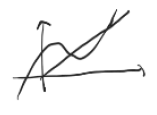
\includegraphics[width=0.3\linewidth]{figures/kein_eindeutiger_fixpunkt}
    \label{fig:kein_eindeutiger_fixpunkt}
\end{figure}



